% !TEX root = ../../../main.tex
% 来源：高中物理甲种本·第三册（电磁·光学·近代物理）
% 章节：光的反射和折射 / 棱镜
% 原始文件：5.tex，行 1129-1141
% 类型：tikz
% ---
	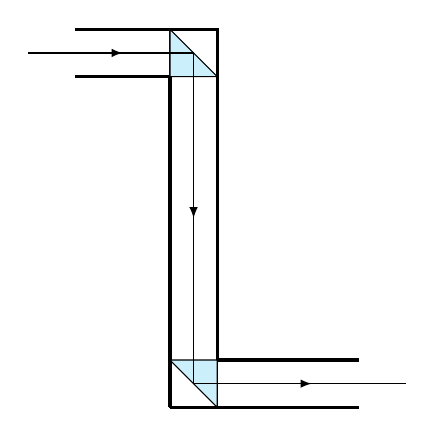
\begin{tikzpicture}[>=latex, scale=1.2]
	\draw (0,0) rectangle (.5, 4);
	\draw [very thick](0,0)--(2,0);  \draw [very thick](.5,0.5)--(2,0.5);
\draw [very thick](0,0)--(0,3.5)--(-1,3.5);  \draw [very thick](.5,0.5)--(.5,4)--(-1,4);
	%\draw (0,4)--(-2,4);  \draw (0,3.5)--(-2,3.5);
\draw [fill=cyan!20](0,0.5)--(.5,.5)--(.5,0)--(0,0.5);
\draw [fill=cyan!20](0,4)--(0,3.5)--(.5,3.5)--(0,4);

\draw(-1.5,3.75)--(.25,3.75)--(0.25,.25)--(2.5,.25);
\draw[->](-1,3.75)--(-.5,3.75);
\draw[->](.25,3.75)--(.25,2);
\draw[->](0.25,.25)--(1.5,.25);
	\end{tikzpicture}
